\documentclass{article}
\usepackage[utf8]{inputenc}

\title{Software Failure and Reliability Assessment Tool: Report}
\author{jesh}
\date{September 01, 2020}

\usepackage{graphicx}
\begin{document}
\maketitle




\section{Data Selection and Analysis}
\subsection{Sampling the input SYS1 data}
The table below shows the first 15 points of the input SYS1 data. `FC' and `CFC' (failure count and cumulative failure count) represent the index of a given failure. `FT' (failure time) represents some units of testing time for which a failure will occur at. `IF' (inter-failure time) represents the amount of time units between two adjacent failures. `FN' denotes the number of a given failure.

\begin{table}[h!]
\centering
\caption{First 15 points of the input data}
\begin{tabular}{lll}
\hline
FN & IF & FT \\ \hline
1 & 3 & 3 \\
2 & 30 & 33 \\
3 & 113 & 146 \\
4 & 81 & 227 \\
5 & 115 & 342 \\
6 & 9 & 351 \\
7 & 2 & 353 \\
8 & 91 & 444 \\
9 & 112 & 556 \\
10 & 15 & 571 \\
11 & 138 & 709 \\
12 & 50 & 759 \\
13 & 77 & 836 \\
14 & 24 & 860 \\
15 & 108 & 968 \\
\hline
\end{tabular}
\end{table}



\newpage
\subsection{Cumulative Failures}
The following figure shows the SYS1 data as the cumulative number of failures (`FN') detected as a function of test time (`FT'). An increasing trend indicates periods where more faults are detected. Ideally, the cumulative number of failures will plateau to a horizontal line, indicating the occurrence of zero new faults.

\begin{figure}[h!]
\centering
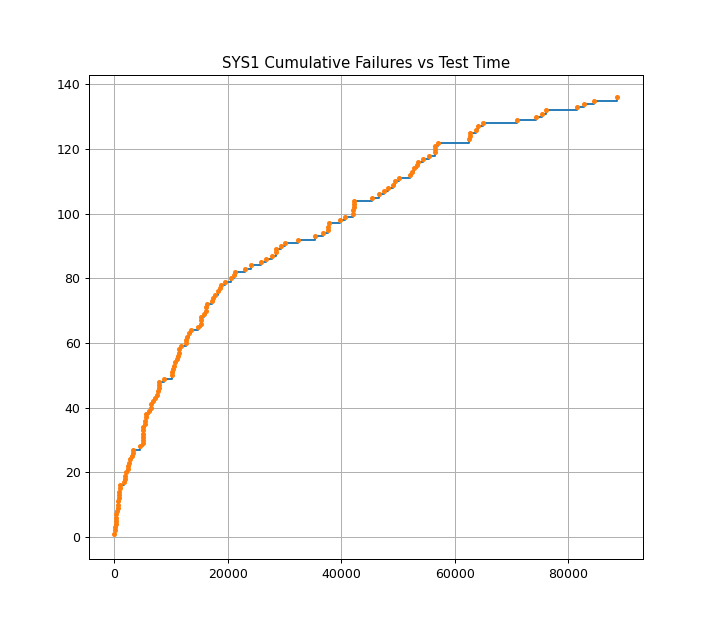
\includegraphics[width=\textwidth]{cfplot1.png}
\caption{Cumulative Failures vs. Cumulative Test Time}
\label{fig:cfplot}
\end{figure}



\newpage
\subsection{Inter-failure Time}
The following figure shows the SYS1 inter-failure times (i.e. times between failures, `IF') as a function of testing time (`FT'). An increasing trend indicates periods where fewer faults are detected. Ideally, the inter-failure time increases maximally, indicating the detection of zero new failures.

\begin{figure}[h!]
\centering
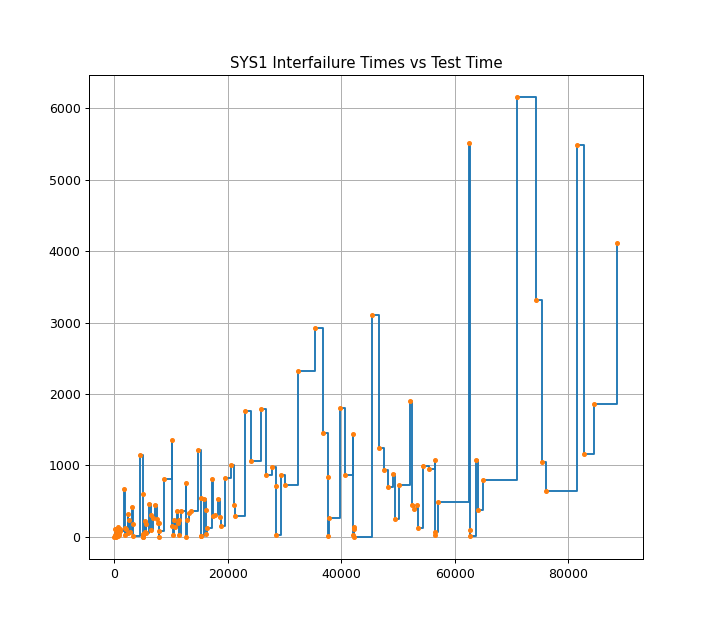
\includegraphics[width=\textwidth]{ifplot1.png}
\caption{Inter-failure Time vs. Cumulative Test Time}
\label{fig:ifplot}
\end{figure}



\newpage
\subsection{Failure Intensity}
The following figure shows the SYS1 data as the number of faults per unit time versus testing time (`FT'). A decreasing trend indicates periods of fewer fault detection. Ideally, the failure intensity should approach zero.

\begin{figure}[h!]
\centering
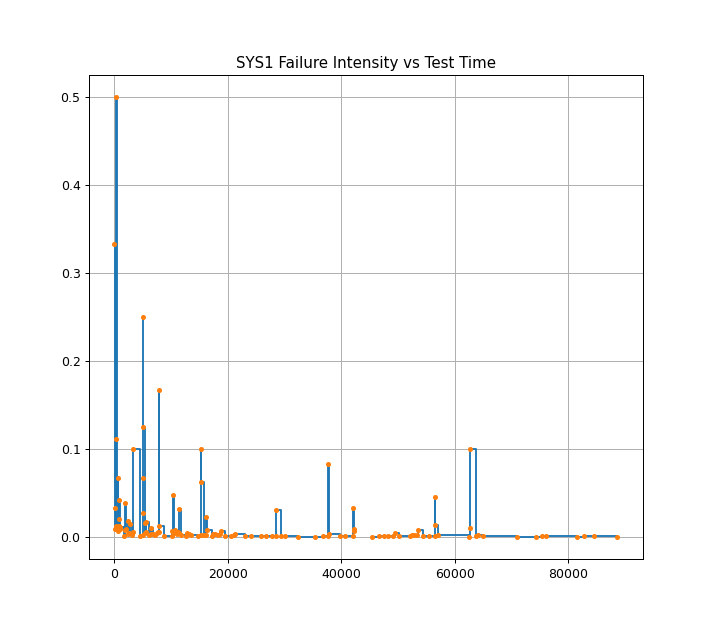
\includegraphics[width=\textwidth]{fiplot1.png}
\caption{Failure Intensity vs. Cumulative Test Time}
\label{fig:fiplot}
\end{figure}



\newpage
\subsection{Laplace Trend Test}
The following figure shows the Laplace test statistic for reliability growth as a function of cumulative test time (FT). A decreasing trend indicates reliability growth, while an increasing trend indicates reliability deterioration. The Laplace test statistic on the y-axis corresponds to the critical values of a normal distribution. This means that if the trend falls below a specific level, then we cannot reject the null hypothesis that the failure data suggests reliability growth at a specified level of confidence. The six black dot-dash style
lines correspond to the 90\%, 95\%, 99\%, 99.9\%, 99.9999\%, and 99.999999\% confidence levels respectively. The red line is user-specified and has been set to 90\%. Reliability growth is desired because software reliability growth models assume curves that exhibit increasing inter-failure times. If reliability growth is not present than the model fitting step may fail or produce predictions that are inaccurate. Therefore, the Laplace test statistic provides an objective quantitative measure for the analyst to decide if predictions may or may not be accurate.


\begin{figure}[h!]
\centering
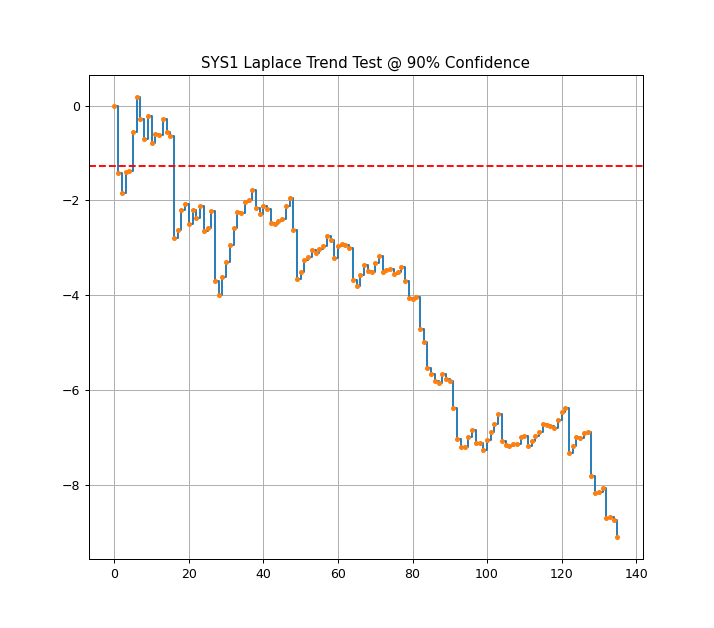
\includegraphics[width=0.75\textwidth]{lapplot1.png}
\caption{Laplace Trend Test at 90\% Confidence, SYS1}
\label{fig:lapplot}
\end{figure}



\newpage
\subsection{Running Arithmetic Average}
The running arithmetic average plots the average of the first k inter-failure times. An increasing trend indicates reliability growth, while a decreasing trend indicates reliability deterioration. This intuitively displays the direct relationship between increasing inter-failure times and the presented average.



\begin{figure}[h!]
\centering
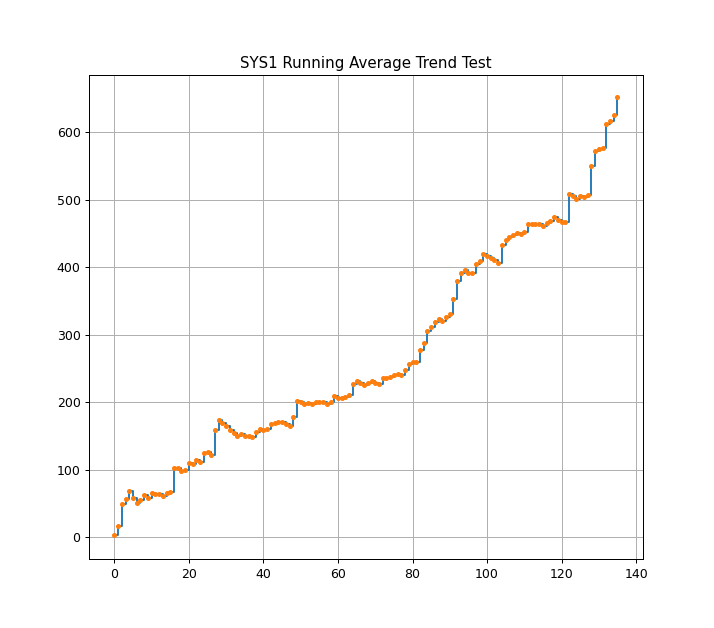
\includegraphics[width=\textwidth]{avgplot1.png}
\caption{Running Arithmetic Average Test, SYS1}
\label{fig:avgplot}
\end{figure}



\newpage



\section{Apply Models to Data}
\subsection{Cumulative Failures}
The following figure shows the fit of Geometric and Jelinski-Moranda models to the cumulative number of failures detected in the SYS1 data. The original data is also shown.



\begin{figure}[h!]
\centering
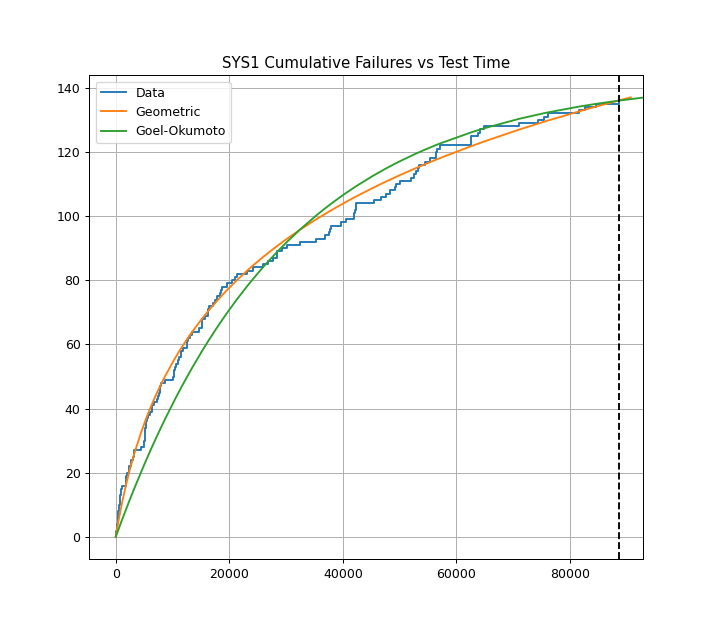
\includegraphics[width=\textwidth]{cfplot2.png}
\caption{Cumulative Failures vs. Cumulative Test Time}
\label{fig:mcfplot}
\end{figure}



\newpage

\subsection{Inter-failure Time}
The following figure shows the fit of Geometric and Jelinski-Moranda models to the inter-failure times in the SYS1 data. The original data is also shown.

\begin{figure}[h!]
\centering
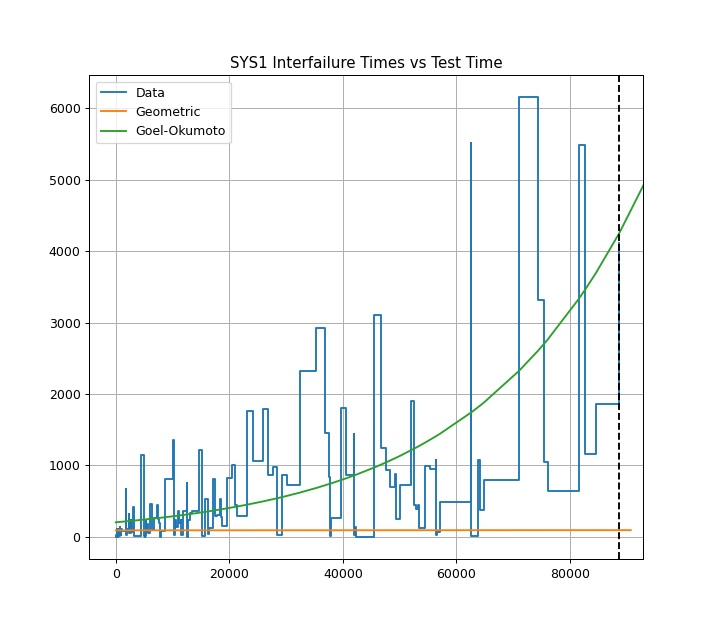
\includegraphics[width=\textwidth]{ifplot2.png}
\caption{Inter-failure Times vs. Cumulative Test Time}
\label{fig:mifplot}
\end{figure}



\newpage

\subsection{Failure Intensity}
The following figure shows the fit of Geometric and Jelinski-Moranda models to the failure intensity of the SYS1 data. The original data is also shown.

\begin{figure}[h!]
\centering
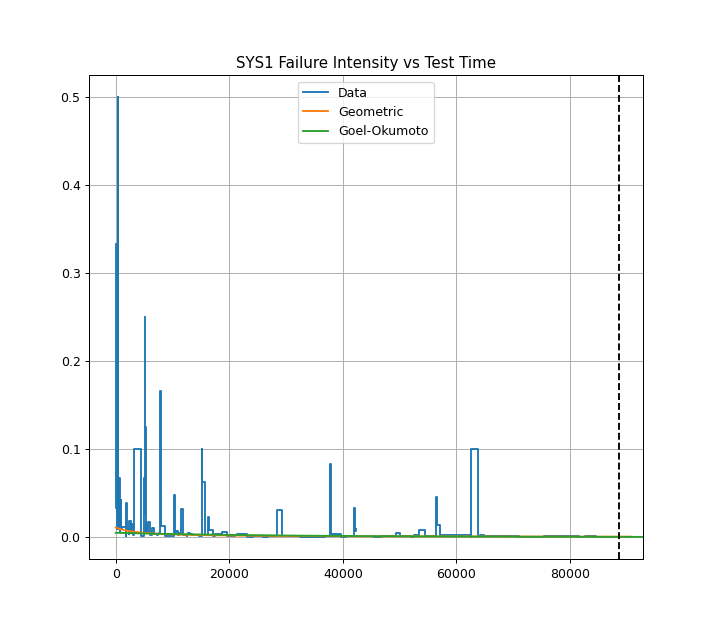
\includegraphics[width=\textwidth]{fiplot2.png}
\caption{Failure Intensity vs. Cumulative Test Time}
\label{fig:mfiplot}
\end{figure}



\newpage

\subsection{Reliability Growth}
The following figure shows the reliability growth curve for the fit of the Geometric and Jelinski-Moranda models to the SYS1 data. This plot indicates a model's prediction that the software will be reliable (i.e. exhibit zero failures) for a duration of 4116 time units, as a function of testing time (`FT'). Assessing a model's reliability is a subjective choice made by the analyst, aided by statistical measures of goodness of fit. Omitting a reliability estimate within a report may be suggested by Laplace test statistic lacking reliability growth.

\begin{figure}[h!]
\centering
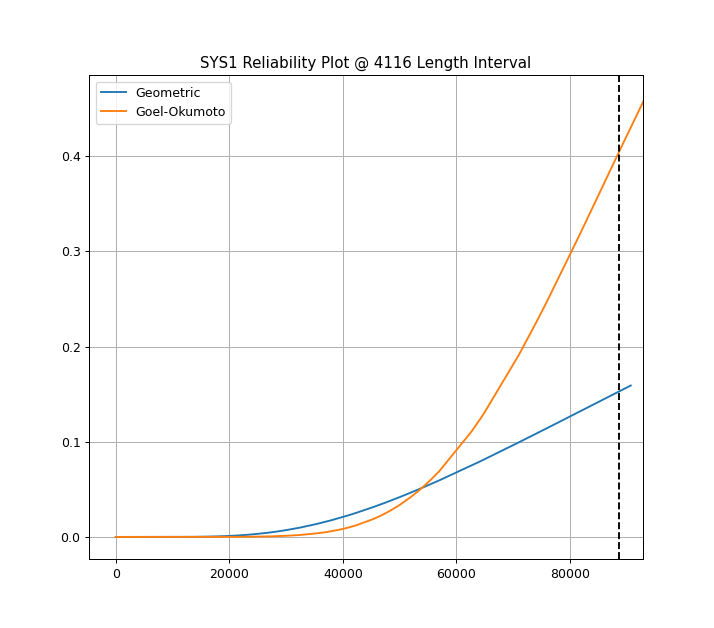
\includegraphics[width=\textwidth]{relplot2.png}
\caption{Reliability Growth vs. Cumulative Test Time}
\label{fig:relplot}
\end{figure}


\newpage


\section{Querying Model Results}
The following table shows inferences enabled by the models, including the time to achieve a reliability of 95\% (i.e. the probability of zero failures for 4116 time units), plus the expected number of failures in the next 4116 and the expected time to observe an additional 10 failures.


\begin{table}[h!]
\centering
\caption{Model Result Query}
\begin{tabular}{llll}
\hline
   & Time, $R=$ 95\% & Failures, $t =$ 4116  & Time, 10 Failures \\ \hline

\hline
\end{tabular}
\end{table}


\newpage


\section{Model Evaluation}
The following table shows the measures of goodness of fit computed for the Geometric and Jelinski-Moranda models. The Aiaike Information Criterion (`AIC') is an information theoretic measure. Lower values are preferred. The  model achieved the lowest AIC with SYS1 data. A difference of 2.0 or more in the AIC values of two models indicates a significant statistical preference. The Predictive Sum of Squares Error (`PSSE') used 90\% of the SYS1 data to fit the models and computed the sum of squares between the remaining 10\% of the data not used to fit the models. Lower values are preferred. The  model achieved the lowest PSSE value on the SYS1 data. The measure of goodness of fit can help select a model, but the choice is ultimately subjective for the analyst.

\begin{table}[h!]
\centering
\caption{Model Evaluation}
\begin{tabular}{lll}
\hline
 &  Akaike Information Criterion & Predictive SSE, 90\% Data \\ \hline

\hline
\end{tabular}
\end{table}

\end{document}
